\documentclass[tikz,border=2mm]{standalone}
\usetikzlibrary{positioning,arrows.meta,calc,decorations.pathreplacing,shapes.geometric,fit}
\definecolor{flowblue}{HTML}{DAE8FC}\definecolor{flowblueline}{HTML}{6C8EBF}
\definecolor{flowgreen}{HTML}{D5E8D4}\definecolor{flowgreenline}{HTML}{82B366}
\definecolor{flowpurple}{HTML}{E1D5E7}\definecolor{flowpurpleline}{HTML}{9673A6}
\definecolor{flowgrey}{HTML}{F5F5F5}\definecolor{flowgreyline}{HTML}{999999}
\begin{document}
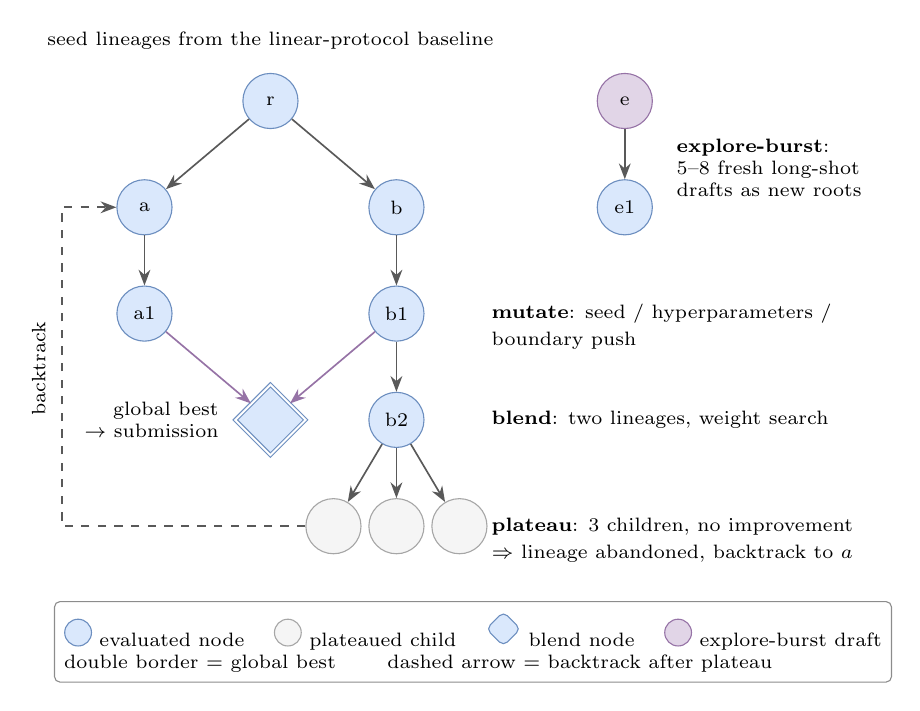
\begin{tikzpicture}[
  font=\footnotesize,
  tn/.style={circle, draw=flowblueline, fill=flowblue, inner sep=0pt, minimum size=7mm,
             font=\scriptsize},
  bn/.style={tn, draw=flowpurpleline, fill=flowpurple},
  pl/.style={tn, draw=black!35, fill=flowgrey, text=black!45},
  bl/.style={tn, diamond, minimum size=9mm},
  te/.style={-{Stealth[length=2mm]}, semithick, black!65},
  lab/.style={font=\scriptsize, inner sep=1.5pt}
]
% ----- lineage a and lineage b, grown from the root -----
\node[tn] (r)  at (3.1,0)     {r};
\node[tn] (A)  at (1.5,-1.35)  {a};
\node[tn] (B)  at (4.7,-1.35)  {b};
\node[tn] (A1) at (1.5,-2.7)   {a1};
\node[tn] (B1) at (4.7,-2.7)   {b1};
\node[tn] (B2) at (4.7,-4.05)  {b2};
\node[pl] (c1) at (3.9,-5.4)   {};
\node[pl] (c2) at (4.7,-5.4)   {};
\node[pl] (c3) at (5.5,-5.4)   {};
% ----- blend node = global best -----
\node[bl, double, double distance=0.7pt] (bd) at (3.1,-4.05) {};
% ----- explore-burst draft as a new root -----
\node[bn] (e)  at (7.6,0)      {e};
\node[tn] (e1) at (7.6,-1.35)  {e1};
\foreach \a/\b in {r/A, r/B, A/A1, B/B1, B1/B2, B2/c1, B2/c2, B2/c3, e/e1}{\draw[te] (\a) -- (\b);}
\draw[te, flowpurpleline] (B1) -- (bd);
\draw[te, flowpurpleline] (A1) -- (bd);
% ----- backtrack: the plateaued lineage is abandoned -----
\draw[te, dashed] (c1.west) -- (0.45,-5.4) -- (0.45,-1.35) -- (A.west);
\node[lab, rotate=90, anchor=south] at (0.3,-3.4) {backtrack};
% ----- annotations -----
\node[lab, anchor=south] at (3.1,0.6)   {seed lineages from the linear-protocol baseline};
\node[lab, anchor=west] at (5.85,-2.7)  {\textbf{mutate}: seed / hyperparameters /};
\node[lab, anchor=west] at (5.85,-3.05) {boundary push};
\node[lab, anchor=west] at (5.85,-4.05) {\textbf{blend}: two lineages, weight search};
\node[lab, anchor=west] at (5.85,-5.4)  {\textbf{plateau}: 3 children, no improvement};
\node[lab, anchor=west] at (5.85,-5.75) {$\Rightarrow$ lineage abandoned, backtrack to $a$};
\node[lab, anchor=west, align=left] at (8.2,-0.85) {\textbf{explore-burst}:\\5--8 fresh long-shot\\drafts as new roots};
\node[lab, anchor=east, align=right] at (2.5,-4.05) {global best\\$\to$ submission};
% ----- legend -----
\node[draw=black!45, rounded corners=2pt, inner sep=3.5pt, anchor=north west,
      align=left, font=\scriptsize] at (0.35,-6.35)
  {\tikz\node[tn, minimum size=3.4mm]{};~evaluated node \quad
   \tikz\node[pl, minimum size=3.4mm]{};~plateaued child \quad
   \tikz\node[bl, minimum size=4.4mm]{};~blend node \quad
   \tikz\node[bn, minimum size=3.4mm]{};~explore-burst draft\\
   double border~$=$~global best \qquad dashed arrow~$=$~backtrack after plateau};
\end{tikzpicture}
\end{document}
